\documentclass[]{article}
\usepackage{lmodern}
\usepackage{amssymb,amsmath}
\usepackage{ifxetex,ifluatex}
\usepackage{fixltx2e} % provides \textsubscript
\ifnum 0\ifxetex 1\fi\ifluatex 1\fi=0 % if pdftex
  \usepackage[T1]{fontenc}
  \usepackage[utf8]{inputenc}
\else % if luatex or xelatex
  \ifxetex
    \usepackage{mathspec}
  \else
    \usepackage{fontspec}
  \fi
  \defaultfontfeatures{Ligatures=TeX,Scale=MatchLowercase}
\fi
% use upquote if available, for straight quotes in verbatim environments
\IfFileExists{upquote.sty}{\usepackage{upquote}}{}
% use microtype if available
\IfFileExists{microtype.sty}{%
\usepackage{microtype}
\UseMicrotypeSet[protrusion]{basicmath} % disable protrusion for tt fonts
}{}
\usepackage[margin=1in]{geometry}
\usepackage{hyperref}
\hypersetup{unicode=true,
            pdftitle={Learning Rate Analysis},
            pdfauthor={Sung Jin Hwang},
            pdfborder={0 0 0},
            breaklinks=true}
\urlstyle{same}  % don't use monospace font for urls
\usepackage{color}
\usepackage{fancyvrb}
\newcommand{\VerbBar}{|}
\newcommand{\VERB}{\Verb[commandchars=\\\{\}]}
\DefineVerbatimEnvironment{Highlighting}{Verbatim}{commandchars=\\\{\}}
% Add ',fontsize=\small' for more characters per line
\usepackage{framed}
\definecolor{shadecolor}{RGB}{248,248,248}
\newenvironment{Shaded}{\begin{snugshade}}{\end{snugshade}}
\newcommand{\KeywordTok}[1]{\textcolor[rgb]{0.13,0.29,0.53}{\textbf{#1}}}
\newcommand{\DataTypeTok}[1]{\textcolor[rgb]{0.13,0.29,0.53}{#1}}
\newcommand{\DecValTok}[1]{\textcolor[rgb]{0.00,0.00,0.81}{#1}}
\newcommand{\BaseNTok}[1]{\textcolor[rgb]{0.00,0.00,0.81}{#1}}
\newcommand{\FloatTok}[1]{\textcolor[rgb]{0.00,0.00,0.81}{#1}}
\newcommand{\ConstantTok}[1]{\textcolor[rgb]{0.00,0.00,0.00}{#1}}
\newcommand{\CharTok}[1]{\textcolor[rgb]{0.31,0.60,0.02}{#1}}
\newcommand{\SpecialCharTok}[1]{\textcolor[rgb]{0.00,0.00,0.00}{#1}}
\newcommand{\StringTok}[1]{\textcolor[rgb]{0.31,0.60,0.02}{#1}}
\newcommand{\VerbatimStringTok}[1]{\textcolor[rgb]{0.31,0.60,0.02}{#1}}
\newcommand{\SpecialStringTok}[1]{\textcolor[rgb]{0.31,0.60,0.02}{#1}}
\newcommand{\ImportTok}[1]{#1}
\newcommand{\CommentTok}[1]{\textcolor[rgb]{0.56,0.35,0.01}{\textit{#1}}}
\newcommand{\DocumentationTok}[1]{\textcolor[rgb]{0.56,0.35,0.01}{\textbf{\textit{#1}}}}
\newcommand{\AnnotationTok}[1]{\textcolor[rgb]{0.56,0.35,0.01}{\textbf{\textit{#1}}}}
\newcommand{\CommentVarTok}[1]{\textcolor[rgb]{0.56,0.35,0.01}{\textbf{\textit{#1}}}}
\newcommand{\OtherTok}[1]{\textcolor[rgb]{0.56,0.35,0.01}{#1}}
\newcommand{\FunctionTok}[1]{\textcolor[rgb]{0.00,0.00,0.00}{#1}}
\newcommand{\VariableTok}[1]{\textcolor[rgb]{0.00,0.00,0.00}{#1}}
\newcommand{\ControlFlowTok}[1]{\textcolor[rgb]{0.13,0.29,0.53}{\textbf{#1}}}
\newcommand{\OperatorTok}[1]{\textcolor[rgb]{0.81,0.36,0.00}{\textbf{#1}}}
\newcommand{\BuiltInTok}[1]{#1}
\newcommand{\ExtensionTok}[1]{#1}
\newcommand{\PreprocessorTok}[1]{\textcolor[rgb]{0.56,0.35,0.01}{\textit{#1}}}
\newcommand{\AttributeTok}[1]{\textcolor[rgb]{0.77,0.63,0.00}{#1}}
\newcommand{\RegionMarkerTok}[1]{#1}
\newcommand{\InformationTok}[1]{\textcolor[rgb]{0.56,0.35,0.01}{\textbf{\textit{#1}}}}
\newcommand{\WarningTok}[1]{\textcolor[rgb]{0.56,0.35,0.01}{\textbf{\textit{#1}}}}
\newcommand{\AlertTok}[1]{\textcolor[rgb]{0.94,0.16,0.16}{#1}}
\newcommand{\ErrorTok}[1]{\textcolor[rgb]{0.64,0.00,0.00}{\textbf{#1}}}
\newcommand{\NormalTok}[1]{#1}
\usepackage{graphicx,grffile}
\makeatletter
\def\maxwidth{\ifdim\Gin@nat@width>\linewidth\linewidth\else\Gin@nat@width\fi}
\def\maxheight{\ifdim\Gin@nat@height>\textheight\textheight\else\Gin@nat@height\fi}
\makeatother
% Scale images if necessary, so that they will not overflow the page
% margins by default, and it is still possible to overwrite the defaults
% using explicit options in \includegraphics[width, height, ...]{}
\setkeys{Gin}{width=\maxwidth,height=\maxheight,keepaspectratio}
\IfFileExists{parskip.sty}{%
\usepackage{parskip}
}{% else
\setlength{\parindent}{0pt}
\setlength{\parskip}{6pt plus 2pt minus 1pt}
}
\setlength{\emergencystretch}{3em}  % prevent overfull lines
\providecommand{\tightlist}{%
  \setlength{\itemsep}{0pt}\setlength{\parskip}{0pt}}
\setcounter{secnumdepth}{0}
% Redefines (sub)paragraphs to behave more like sections
\ifx\paragraph\undefined\else
\let\oldparagraph\paragraph
\renewcommand{\paragraph}[1]{\oldparagraph{#1}\mbox{}}
\fi
\ifx\subparagraph\undefined\else
\let\oldsubparagraph\subparagraph
\renewcommand{\subparagraph}[1]{\oldsubparagraph{#1}\mbox{}}
\fi

%%% Use protect on footnotes to avoid problems with footnotes in titles
\let\rmarkdownfootnote\footnote%
\def\footnote{\protect\rmarkdownfootnote}

%%% Change title format to be more compact
\usepackage{titling}

% Create subtitle command for use in maketitle
\newcommand{\subtitle}[1]{
  \posttitle{
    \begin{center}\large#1\end{center}
    }
}

\setlength{\droptitle}{-2em}

  \title{Learning Rate Analysis}
    \pretitle{\vspace{\droptitle}\centering\huge}
  \posttitle{\par}
    \author{Sung Jin Hwang}
    \preauthor{\centering\large\emph}
  \postauthor{\par}
      \predate{\centering\large\emph}
  \postdate{\par}
    \date{3/4/2019}


\begin{document}
\maketitle

\begin{Shaded}
\begin{Highlighting}[]
\KeywordTok{library}\NormalTok{(ggplot2)}
\NormalTok{time_to_fail <-}\StringTok{ }\KeywordTok{read.csv}\NormalTok{(}\StringTok{"time_to_fail.csv"}\NormalTok{)}
\KeywordTok{colnames}\NormalTok{(time_to_fail) <-}\StringTok{ }\KeywordTok{c}\NormalTok{(}\StringTok{"X"}\NormalTok{, }\StringTok{"TimeAtFail"}\NormalTok{)}

\NormalTok{time_to_fail}\OperatorTok{$}\NormalTok{TimeToFail <-}\StringTok{ }\KeywordTok{c}\NormalTok{(}\DecValTok{0}\NormalTok{,}\KeywordTok{diff}\NormalTok{(time_to_fail}\OperatorTok{$}\NormalTok{TimeAtFail))}



\KeywordTok{ggplot}\NormalTok{(}\DataTypeTok{data =}\NormalTok{ time_to_fail, }\KeywordTok{aes}\NormalTok{(}\DataTypeTok{x=}\NormalTok{TimeAtFail, }\DataTypeTok{y=}\NormalTok{TimeToFail)) }\OperatorTok{+}\StringTok{ }
\StringTok{  }\KeywordTok{geom_point}\NormalTok{(}\DataTypeTok{alpha =} \FloatTok{0.5}\NormalTok{) }\OperatorTok{+}
\StringTok{  }\KeywordTok{geom_smooth}\NormalTok{(}\DataTypeTok{se =} \OtherTok{FALSE}\NormalTok{, }\DataTypeTok{col =} \StringTok{"red"}\NormalTok{)}
\end{Highlighting}
\end{Shaded}

\begin{verbatim}
## `geom_smooth()` using method = 'gam' and formula 'y ~ s(x, bs = "cs")'
\end{verbatim}

\includegraphics{analysis_files/figure-latex/unnamed-chunk-1-1.pdf}

\section{Training a deep neural network to play a
game}\label{training-a-deep-neural-network-to-play-a-game}

My project was training a convolutional neural network to play a simple
flash based game called ``Flappy Bird''. The purpose of this project was
to familiarize myself with using Google's Tensoflow package, and the
concept of reinforcement learning. I followed the open git project by
Yen Chen Lin at
\url{https://github.com/yenchenlin/DeepLearningFlappyBird}. This
tutorial will explain the concept of the learning process design, and
usage of Tensorflow function in developing a network.

\section{Convolutional Neural
Network}\label{convolutional-neural-network}

Convolutional neural network, or CNN, is a type of deep neural network
that is commonly applied to analyzing visual imagery. CNNs requires less
pre-processing than other image classification algorithms. The network
learns the features of the image that are usually hand-egineered for
traditional algorithms. This characteristics of CNN in feature design is
a major advantage.

A CNN consists of an input layer, multiple hidden layers, and an output
layer. The hidden layers of a CNN may be convolutional layers,
activation functions (Common function is Rectified Linear Unit (RELU)
function), max pooling layers, fully connected layers and normalization
layers.

More detailed tutorials on convolutional neural network can be found in:
\url{https://towardsdatascience.com/a-comprehensive-guide-to-convolutional-neural-networks-the-eli5-way-3bd2b1164a53}

\section{Reinforcement Learning}\label{reinforcement-learning}

This project uses one class of reniforcement learning. Reinforcement
learning is a learning design that's similar to Pavlov's Dog experiment,
where dog was given rewards based on their action in repetitive manner.
Reinforcement learning will generate a state where network makes a
decision based on that state. The set of rules will decide whether the
network received a positive reward or negative reward as a feedback.
Based on the reward, the network will adjust it's values to make better
decisions for the next state.

\section{DeepQLearning}\label{deepqlearning}

Combining the reinforcement learning to CNN, comes the deep Q learning.
In Q-learning, we define Q as a function \(Q(s,a)\) which represents the
maximum discounted future reward when the network performs action \(a\)
in the state \(s\).

\[Q(s_t,a_t) = max R_{t+1}\] In the context of this project, we can
think of Q as best possible score from performing one action in certain
game state. Now we just have to choose the action that yields the
highest Q value for each state. Defining the Q function, we can use the
Bellman Equation. \[Q(s,a) = r + \gamma*max_{a'}Q(s',a')\] Here, \(s'\)
is the one step future state and \(a'\) is the one step future action.
Logically, this function means maximum future reward for this state and
action is the immediate reward plus maximum future reward for the next
state.

We use CNN to implement this Q function.

\begin{figure}
\centering
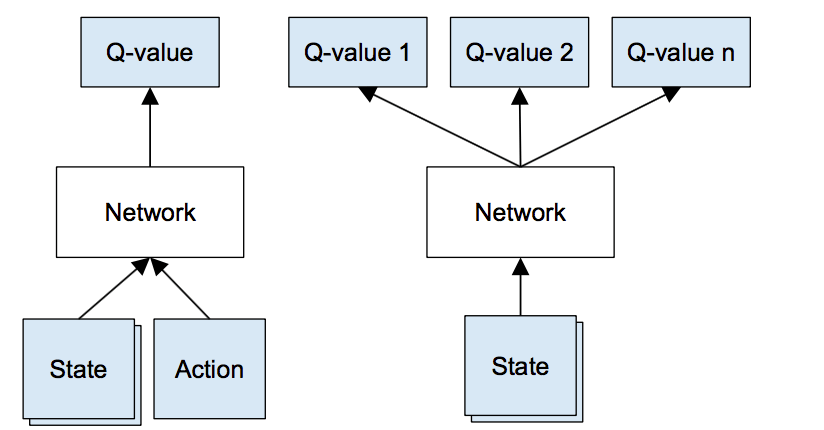
\includegraphics{deep-q-network-example.png}
\caption{Left: Naive formulation of deep Q-network. Right: More
optimized architecture of deep Q-network, used in DeepMind
paper.\n Image Source:
\url{https://www.intel.ai/demystifying-deep-reinforcement-learning/\#gs.ZVqWFqk6}}
\end{figure}

\section{Setting up a network using
Tensorflow}\label{setting-up-a-network-using-tensorflow}

We can think of tensorflow as a package that makes building a neural
network lot easier than doing it without such tools. Lets walk through
some examples.

First we want to install tensorflow.

\begin{Shaded}
\begin{Highlighting}[]
\ExtensionTok{pip}\NormalTok{ install python}
\end{Highlighting}
\end{Shaded}

This should do the work of installing

\begin{Shaded}
\begin{Highlighting}[]
\ImportTok{import}\NormalTok{ tensorflow }\ImportTok{as}\NormalTok{ tf}

\KeywordTok{def}\NormalTok{ conv2d(x, weights, stride):}
    \ControlFlowTok{return}\NormalTok{ tf.nn.conv2d(x, weights, strides }\OperatorTok{=}\NormalTok{ [}\DecValTok{1}\NormalTok{, stride, stride, }\DecValTok{1}\NormalTok{], padding }\OperatorTok{=} \StringTok{"SAME"}\NormalTok{)}

\KeywordTok{def}\NormalTok{ max_pool_2x2(x):}
    \ControlFlowTok{return}\NormalTok{ tf.nn.max_pool(x, ksize }\OperatorTok{=}\NormalTok{ [}\DecValTok{1}\NormalTok{, }\DecValTok{2}\NormalTok{, }\DecValTok{2}\NormalTok{, }\DecValTok{1}\NormalTok{], strides }\OperatorTok{=}\NormalTok{ [}\DecValTok{1}\NormalTok{, }\DecValTok{2}\NormalTok{, }\DecValTok{2}\NormalTok{, }\DecValTok{1}\NormalTok{], padding }\OperatorTok{=} \StringTok{"SAME"}\NormalTok{)}

\KeywordTok{def}\NormalTok{ createNetwork():}
    \CommentTok{# network weights}
\NormalTok{    weights_conv1 }\OperatorTok{=}\NormalTok{ tf.Variable(tf.truncated_normal(shape }\OperatorTok{=}\NormalTok{ [}\DecValTok{8}\NormalTok{, }\DecValTok{8}\NormalTok{, }\DecValTok{4}\NormalTok{, }\DecValTok{32}\NormalTok{], stddev }\OperatorTok{=} \FloatTok{0.01}\NormalTok{))}
\NormalTok{    bias_conv1 }\OperatorTok{=}\NormalTok{ tf.Variable(tf.constant(}\FloatTok{0.01}\NormalTok{, shape }\OperatorTok{=}\NormalTok{ [}\DecValTok{32}\NormalTok{]))}

\NormalTok{    weights_conv2 }\OperatorTok{=}\NormalTok{ tf.Variable(tf.truncated_normal(shape }\OperatorTok{=}\NormalTok{ [}\DecValTok{4}\NormalTok{, }\DecValTok{4}\NormalTok{, }\DecValTok{32}\NormalTok{, }\DecValTok{64}\NormalTok{], stddev }\OperatorTok{=} \FloatTok{0.01}\NormalTok{))}
\NormalTok{    bias_conv2 }\OperatorTok{=}\NormalTok{ tf.Variable(tf.constant(}\FloatTok{0.01}\NormalTok{, shape }\OperatorTok{=}\NormalTok{ [}\DecValTok{64}\NormalTok{]))}

\NormalTok{    weights_conv3 }\OperatorTok{=}\NormalTok{ tf.Variable(tf.truncated_normal(shape }\OperatorTok{=}\NormalTok{ [}\DecValTok{3}\NormalTok{, }\DecValTok{3}\NormalTok{, }\DecValTok{64}\NormalTok{, }\DecValTok{64}\NormalTok{], stddev }\OperatorTok{=} \FloatTok{0.01}\NormalTok{))}
\NormalTok{    bias_conv3 }\OperatorTok{=}\NormalTok{ tf.Variable(tf.constant(}\FloatTok{0.01}\NormalTok{, shape }\OperatorTok{=}\NormalTok{ [}\DecValTok{64}\NormalTok{]))}

\NormalTok{    weights_fc1 }\OperatorTok{=}\NormalTok{ tf.Variable(tf.truncated_normal(shape }\OperatorTok{=}\NormalTok{ [}\DecValTok{1600}\NormalTok{, }\DecValTok{512}\NormalTok{], stddev }\OperatorTok{=} \FloatTok{0.01}\NormalTok{))}
\NormalTok{    bias_fc1 }\OperatorTok{=}\NormalTok{ tf.Variable(tf.constant(}\FloatTok{0.01}\NormalTok{, shape }\OperatorTok{=}\NormalTok{ [}\DecValTok{512}\NormalTok{]))}

\NormalTok{    weights_fc2 }\OperatorTok{=}\NormalTok{ tf.Variable(tf.truncated_normal(shape }\OperatorTok{=}\NormalTok{ [}\DecValTok{512}\NormalTok{, }\DecValTok{2}\NormalTok{], stddev }\OperatorTok{=} \FloatTok{0.01}\NormalTok{))}
\NormalTok{    bias_fc2 }\OperatorTok{=}\NormalTok{ tf.Variable(tf.constant(}\FloatTok{0.01}\NormalTok{, shape }\OperatorTok{=}\NormalTok{ [}\DecValTok{2}\NormalTok{]))}

    \CommentTok{# input layer}
\NormalTok{    s }\OperatorTok{=}\NormalTok{ tf.placeholder(}\StringTok{"float"}\NormalTok{, [}\VariableTok{None}\NormalTok{, }\DecValTok{80}\NormalTok{, }\DecValTok{80}\NormalTok{, }\DecValTok{4}\NormalTok{])}

    \CommentTok{# hidden layers}
\NormalTok{    h_conv1 }\OperatorTok{=}\NormalTok{ tf.nn.relu(conv2d(s, weights_conv1, }\DecValTok{4}\NormalTok{) }\OperatorTok{+}\NormalTok{ bias_conv1)}
\NormalTok{    h_pool1 }\OperatorTok{=}\NormalTok{ max_pool_2x2(h_conv1)}

\NormalTok{    h_conv2 }\OperatorTok{=}\NormalTok{ tf.nn.relu(conv2d(h_pool1, weights_conv2, }\DecValTok{2}\NormalTok{) }\OperatorTok{+}\NormalTok{ bias_conv2)}

\NormalTok{    h_conv3 }\OperatorTok{=}\NormalTok{ tf.nn.relu(conv2d(h_conv2, weights_conv3, }\DecValTok{1}\NormalTok{) }\OperatorTok{+}\NormalTok{ bias_conv3)}

\NormalTok{    h_conv3_flat }\OperatorTok{=}\NormalTok{ tf.reshape(h_conv3, [}\OperatorTok{-}\DecValTok{1}\NormalTok{, }\DecValTok{1600}\NormalTok{])}

\NormalTok{    h_full_connect1 }\OperatorTok{=}\NormalTok{ tf.nn.relu(tf.matmul(h_conv3_flat, weights_fc1) }\OperatorTok{+}\NormalTok{ bias_fc1)}

    \CommentTok{# readout layer}
\NormalTok{    Q }\OperatorTok{=}\NormalTok{ tf.matmul(h_full_connect1, weights_fc2) }\OperatorTok{+}\NormalTok{ bias_fc2}

    \ControlFlowTok{return}\NormalTok{ s, Q}
\end{Highlighting}
\end{Shaded}


\end{document}
